Grundsätzlich versprechen sich die Autoren von richtig implementierter Parallelisierung einen messbaren Zusammenhang von der Anzahl der verwendeten Rechenknoten und der resultierenden Laufzeit.
Um diese These zu überprüfen, und weitere mögliche Zusammenhänge zu erfassen, wurden im Rahmen der Arbeit umfassende Laufzeitmessungen durchgeführt.
Um Vergleichbarkeit herzustellen, wurden alle Messungen innerhalb kürzester Zeit am gleichen Tag vorgenommen. Aufgrund beschränkter Zeit wurde eine Stichprobengröße von $n = 10$ Messungen pro Messklasse gewählt.
Es sei angemerkt: wünschenswert und für eine statistisch fundierter Aussage notwendig wäre das fünf bis zehnfache hiervon. \\
Die Messklassen werden hier über die Anzahl der verwendeten Rechenknoten festgelegt; für die Auswertung wurden Messungen mit einem bis sieben Rechenknoten durchgeführt.
Gemessen wird jeweils die benötigte Laufzeit, eine wohldefinierte und unveränderliche Datei bestehend aus einer großen Zahl von Wörtern zu sortieren.
Eine Messergebnis ist die mithilfe der Standard Template Bibliothek std::chrono gemessene Zeit, welche im Programmablauf des Master-Knotens zwischen dem Zeitpunkt unmittelbar vor der Verteilung der Teilelemente 
des zu sortierenden Textes an die Slave-Knoten und dem Zeitpunkt unmittelbar nach dem Zusammenführen der Ergebnisse der Slave-Rechenknoten verstreicht.
Das arithmetische Mittel sowie die Standardabweichung der Messreihen sind in Tabelle 1 aufgeführt.
\begin{table}
    \centering
    \caption{Zeitmessungen mit verschiedenen Anzahlen an Rechenknoten}
    \label{zeiten_tabelle}
    \begin{tabular}{l|lllllll}
    \textbf{Anzahl der Rechenknoten}  & \textbf{1} & \textbf{2} & \textbf{3} & \textbf{4} & \textbf{5} & \textbf{6} & \textbf{7}  \\ 
    \hline\hline
    \%\textbackslash{}bar\{t\}\$ [ms] & 4382.9     & 2413.7     & 2148.5     & 1728.6     & 1715.9     & 1621.6     & 1574.6      \\
    \$\textbackslash{}sigma\$ [ms]    & 491.2      & 128.0      & 113.9      & 72.2       & 70.9       & 62.3       & 112.4      
    \end{tabular}
\end{table}
Bei der Messreihe mit genau einem Rechenknoten ist eine erhöhte Unsicherheit zu erkennen. Dennoch ist der Mittelwert signifikant höher als bei allen anderen 
Messungen mit einer Rechenknotenanzahl größer eins. Bei den Anzahlen vier, fünf und sechs ist eine im Vergleich geringe Abweichung festzustellen. Diese Werte haben eine entsprechend hohe 
Aussagekraft. Interessanterweise sind die Mittelwerte der Zeiten ab einer Rechenknotenanzahl von 4 sehr nah beieinander. Daher kann mit den vorliegenden Daten keine statistisch begründete Aussage getroffen werden, ob sich die Rechenzeit ab einer Knotenzahl von 4 noch messbar verändert. Hierfür liegen die Messungen zu nah beieinander. Der scheinbar deutlich niedrigere Mittelwert der 7. Messung wird durch eine
höhere Messunsicherheit relativiert.
\\
Eine umfassendere Darstellung der Daten erfolgt mithilfe eines Whiskers Plots, auch Kastenschaubild genannt (Abbildung X). Auch hier ist die vermutete, anfängliche und deutliche 
Absenkung der Laufzeiten über die Anzahl der Rechenknoten zu erkennen. Ebenfalls fällt ein starker Ausreißer bei der Knotenzahl eins auf. Auch bei Knotenzahlen zwei, vier und sechs 
gibt es solche Ausreißer. Interessanterweise gibt es gerade bei den Knotenzahlen vier und sechs, welche eine relativ geringe Standardabweichung aufweisen, ebenfalls Ausreißer nach oben. 
Im Kontext der niedrigen Standardabweichung bedeutet das einerseits, dass die restlichen Messwerte dieser Messreihen besonders konsistent sind. Andererseits könnte dies ein Hinweis darauf sein, dass die gemessenen Zeiten durch Zufall besonders konsistent und niedrig ausgefallen sind.
\begin{figure}[!t]
    \centering
    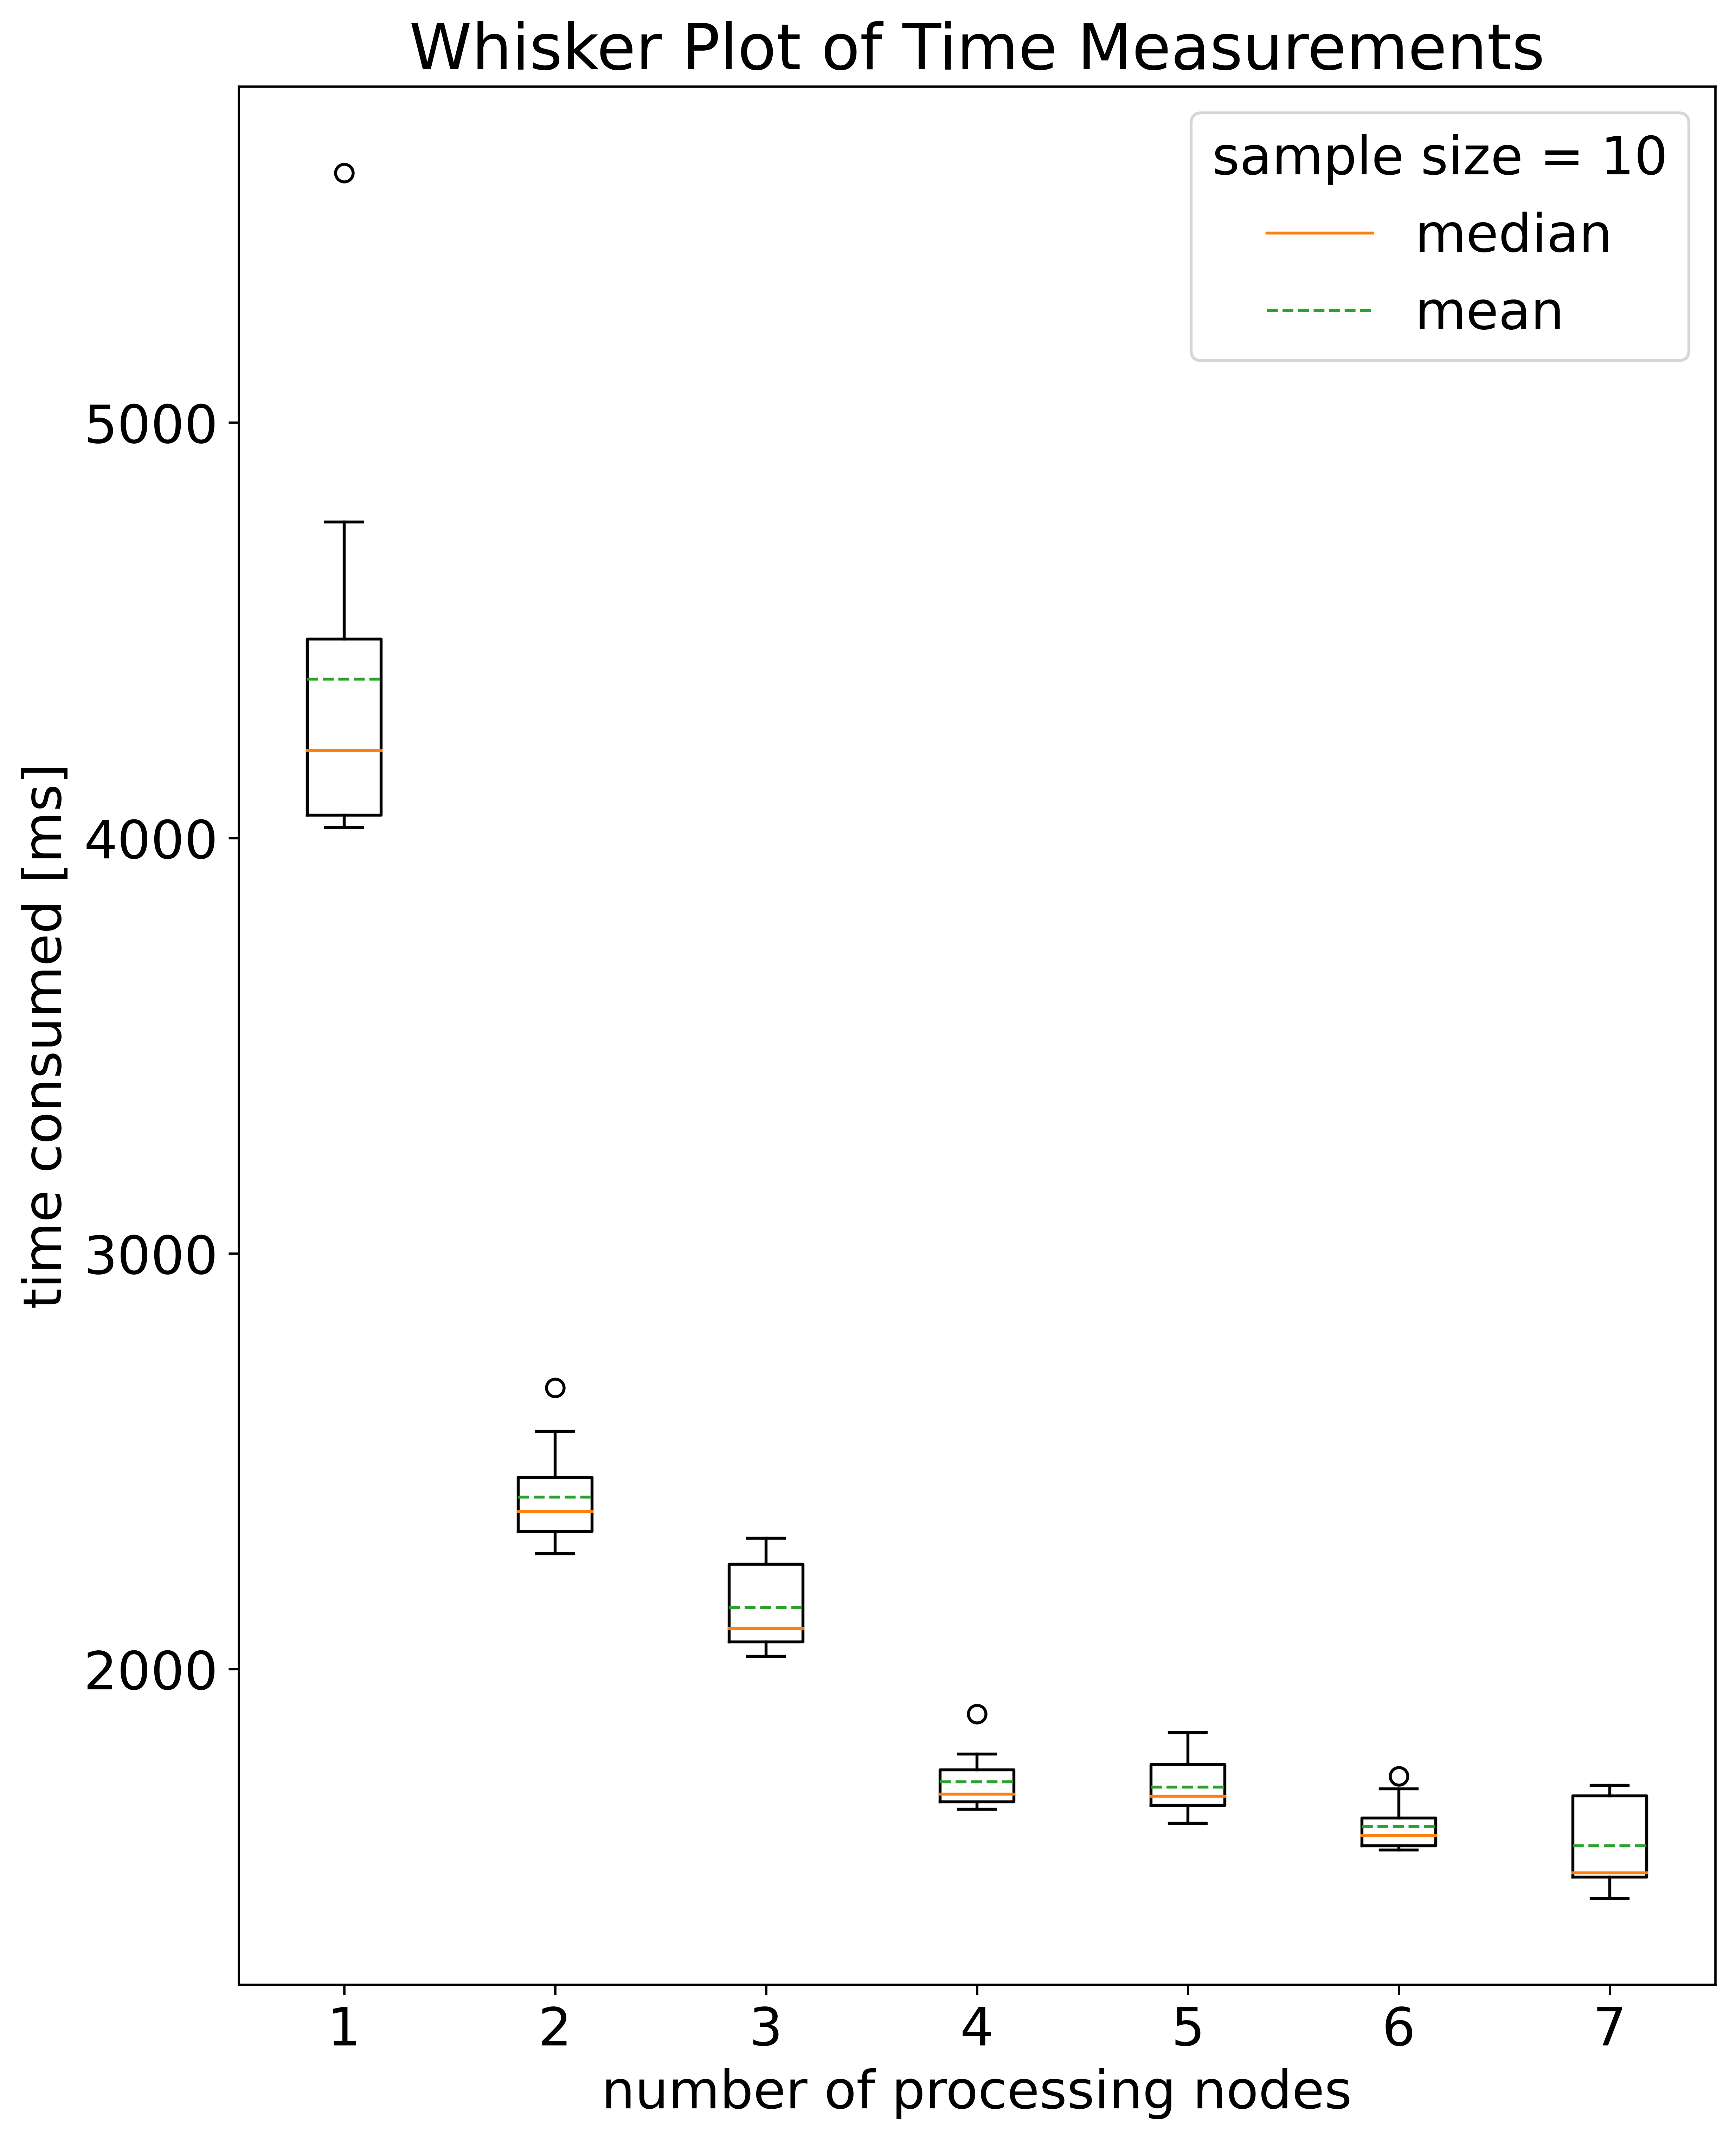
\includegraphics[width=3.5in]{boxplots.png}
    \caption{Cpation is already in picture!}
    \label{boxplot_times}
\end{figure}
\\
So lassen die beobachteten Phänomene insgesamt darauf schließen, dass die Parallelisierung in ihrer für das Projekt durchgeführten Implementierung eine signifikante Absenkung der Laufzeit von bis zu einer Größenordnung von 60\% mit sich bringt. Dieser Effekt ist jedoch stark begrenzt und flacht mit einer steigenden Rechenknotenanzahl schnell ab bzw. verschwindet gänzlich. Die Effizienz pro Rechenknoten nimmt damit bei steigender Anzahl von Rechenknoten schnell ab.
Für genauere Aussagen ist eine größere Anzahl an Messungen pro Messklasse für nötig.
\\
Eine Deutung für die Beobachteten Ergebnisse: die Rechenknoten in der Cloud sind mittels Ethernet miteinander verbunden, was das Senden und Empfangen von Nachrichten erstens nicht zeitlich deterministisch und zweitens anfällig für unregelmäßige und längere Laufzeiten macht. Offenbar bewegt sich bei der betrachteten Dateigröße das Senden und Empfangen von Nachrichten an mehr Knoten ab einer Knotenzahl von ca. vier in einer ähnlichen Größenordnungen wie der Laufzeitgewinn, welcher dadurch entsteht, dass ein Rechenknoten nur eine geringere Anzahl an Arbeit (Wörter sortieren) hat. Die Autoren vermuten, dass bei einer deutlich größeren Datei (mit mehr Wörtern), ein Laufzeitgewinn auch bei größeren Knotenzahlen zu messen sein wird.